\documentclass[aps,pra,groupedaddress,twocolumn,notitlepage,superscriptaddress,10pt]{revtex4-1}

%\usepackage[utf8]{inputenc}
%\usepackage{mathpazo}
%\usepackage{mathptmx}
%\usepackage{tgpagella}
%\usepackage{tgtermes}

\usepackage{float}
\usepackage{graphicx}  % needed for figures
\usepackage{xcolor}
\usepackage{dcolumn}   % needed for some tables
\usepackage{bm}        % for math
\usepackage{braket}
\usepackage{amssymb}   % for math
\usepackage{epstopdf}
\usepackage{xfrac}

\usepackage{amsmath}
\usepackage{amsthm}
\usepackage{amsfonts}
\usepackage{bbm}
% configure hyperref to remove ugly boxes from links
\definecolor{darkblue}{rgb}{0.1,0.2,0.6}
\definecolor{darkred}{rgb}{0.8,0.1,0.2}
\usepackage[colorlinks,citecolor=darkblue,linkcolor=darkblue,urlcolor=darkblue]{hyperref} 
\usepackage{tikz}
\usepackage{enumerate}
\usepackage{setspace}
\usepackage{url}  % This makes \url work
\usepackage{mathrsfs}

\def\ua{\uparrow}
\def\da{\downarrow}
\newcommand{\rT}{{\rho^{T_2}} }
\newcommand{\rTa}{{\rho^{T_2}_A} }
\newcommand{\rTc}{{\rho^{T_2}} }
\newcommand{\Hi}{\mathcal{H}}
\newcommand{\Ni}{\mathcal{N}}
\newcommand{\C}{\mathbb{C}}
\newcommand{\Z}{\mathbb{Z}}
\newcommand{\R}{\mathbb{R}}
\newcommand{\I}{\mathbb{I}}
\newcommand{\Rp}{{\cal R}_\text{part}}
\newcommand{\sgn}{\text{sign}}

\newcommand{\xv}{\textbf{x}}
\newcommand{\ev}{\textbf{e}}
\newcommand{\iv}{\textbf{i}}
\newcommand{\jv}{\textbf{j}}
\newcommand{\Tr}{\text{Tr}}
\newcommand{\tr}{\text{Tr}}
\newcommand{\del}{\nabla}
\newcommand{\norm}[1]{\left\lVert#1\right\rVert}

\newcommand{\vac}{\ket{0}\bra{0}}
\newcommand{\kvac}{\ket{\text{vac}}}
\newcommand{\bvac}{\bra{\text{vac}}}
\newcommand{\bigket}[1]{ {\big|{#1}\big\rangle} }
\newcommand{\Bigket}[1]{ {\Big|{#1}\Big\rangle} }
\newcommand{\bigbra}[1]{ {\big\langle{#1}\big|} }
\newcommand{\Bigbra}[1]{ {\Big\langle{#1}\Big|} }


\usepackage{tikz}
\usetikzlibrary{positioning}
\usetikzlibrary{patterns}

%\usepackage{tikzit}

\newcommand*{\HS}[1]{\textcolor{blue}{[HS: #1]}}
\newcommand*{\SL}[1]{\textcolor{magenta}{[SL: \textsf{#1}]}}
\newcommand*{\change}[2]{{\color{red}\sout{#1}}{ \color{blue}#2}}

\begin{document}

\title{Entanglement transitions in random pure states}
\author{Hassan Shapourian%
%  \thanks{Electronic address: \texttt{hassan.shapp@gmail.com}}
  }
% \affiliation{Department of Physics, Harvard University, Cambridge, MA~02138, USA}
% \affiliation{Department of Physics, Massachusetts Institute of Technology,
% Cambridge, MA~02139, USA}
\author{Jonah Kudler-flam%
}
% \affiliation{Kadanoff Center for Theoretical Physics, University of Chicago, IL 60637, USA}


\date{\today}

\begin{abstract}
In this paper, we use large-$N$ perturbation theory to compute the entanglement negativity of random induced mixed states. Our result reproduces the two well-known limits: volume law states and separable states. We also find that the volume law states can be further divided into two categories in terms of subsystem-size scaling  of the entanglement  negativity: a linear scaling phase, where ${\cal E}\sim V_{A_1}$, and a saturated phase, where ${\cal E}\sim (V_{A}-V_B)/2$, which  is independent of individual subsystem sizes $V_{A_1}$ and $V_{A_2}$. In the latter case, the spectral density can be well-approximated by a semi-circle law. We show that the large-$N$ perturbation theory results match with those of the random matrix simulations.
Our finding indicates that the average logarithmic negativity behaves very similar to the $1/2$-R\'enyi mutual information.
\end{abstract}

\maketitle

\section{Introduction}

Random pure states represent typical volume law entangled  (thermal) pure states. Their virtue is that they are described by Wishart random matrix theory and hence, various well-established random matrix theory tools are available to carry out calculations on them.

In this paper, we use the large-N perturbation theory which was recently developed by one of us to compute the spectral density of partial transpose and characterize the reduced density matrix in several limits. The result is summarized in Fig.~\ref{fig:phasediag}.

\begin{figure}
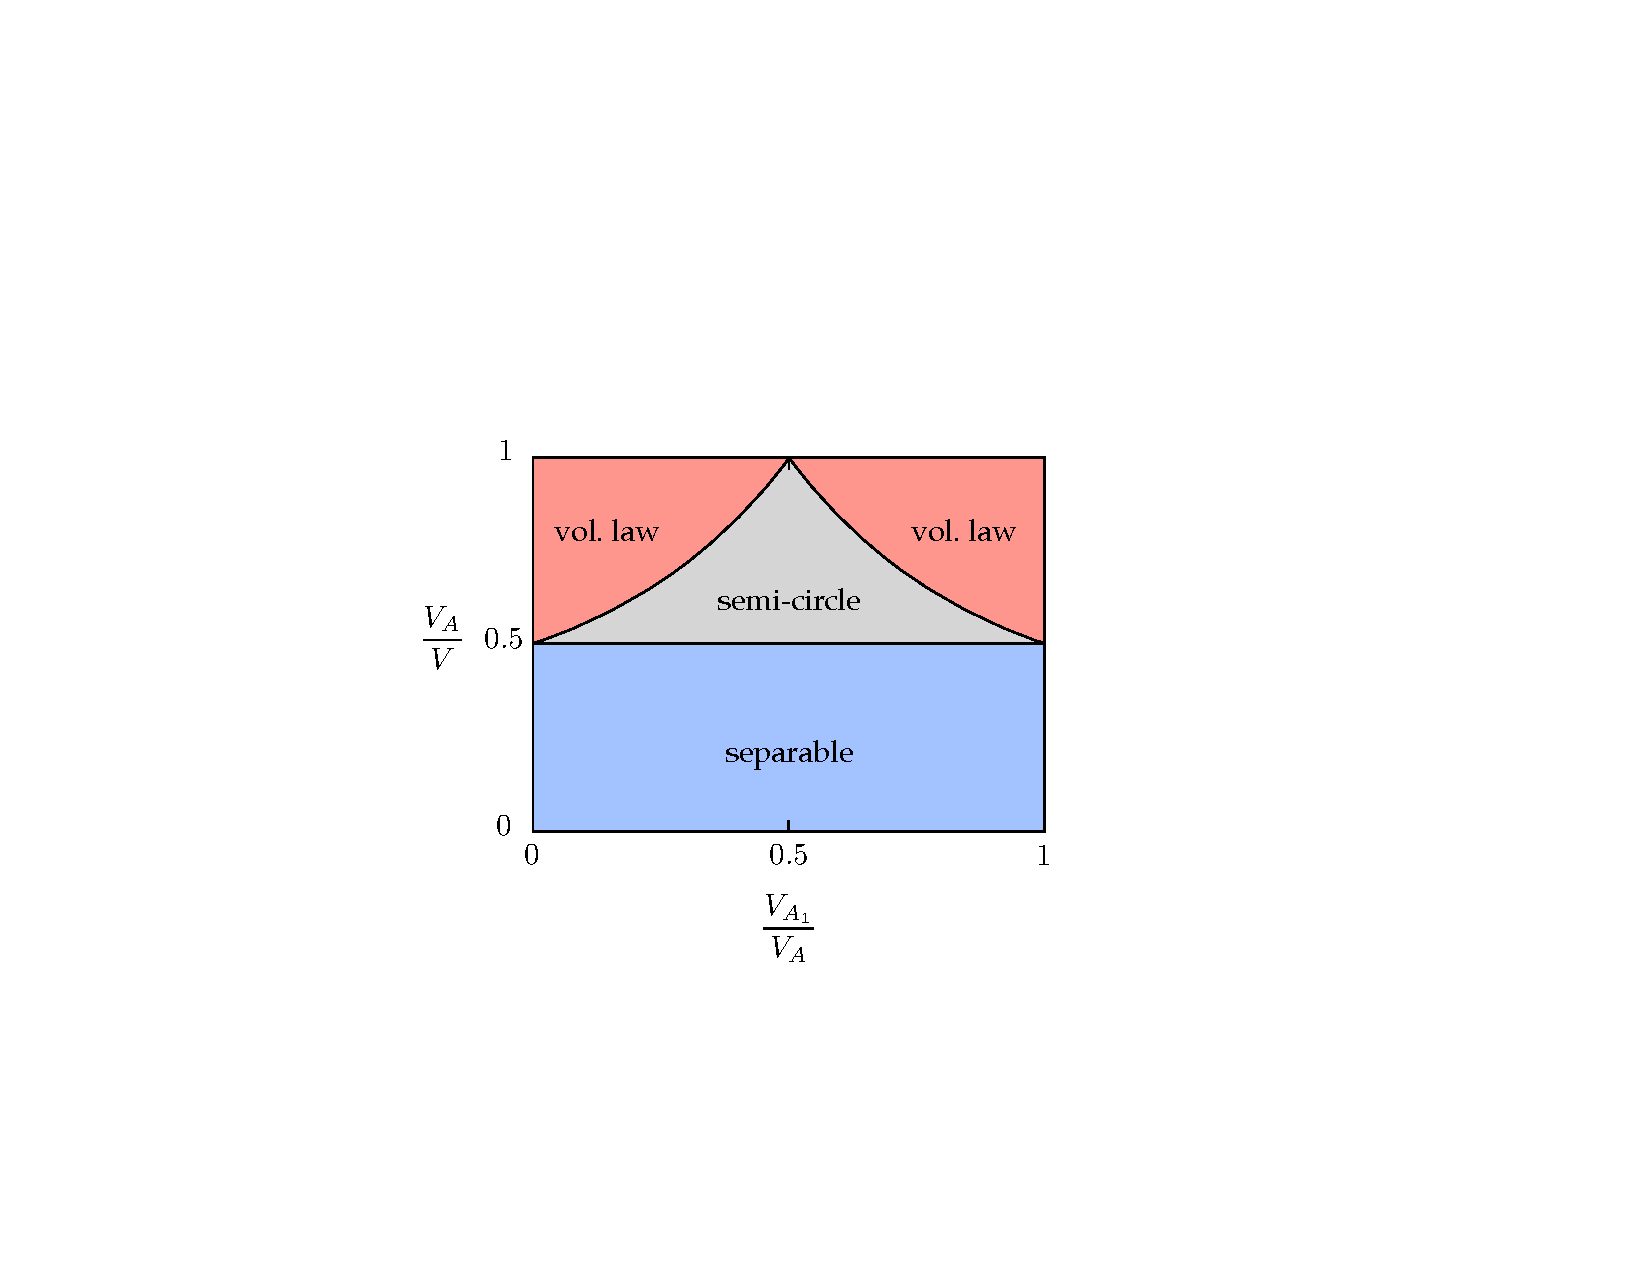
\includegraphics[scale=0.6]{images/phase_diag.pdf}
\caption{\label{fig:phasediag} Phase diagram of reduced density matrix obtained from random pure states (or Page states).}
\end{figure}

\section{Large-N perturbation theory}
In this section, we use graphical representation of a partially transposed random mixed state to  compute its momets  and eventually derive the corresponding resolvent function and the spectral density.


\subsection{Moments of partial transpose}

Let us look at the dominant diagrams deep in the NPT limit, $L_A\gg L_B$, when one subsystem ($A_1$ or $A_2$) is much larger than the other. 
\begin{align}
    \braket{\Tr \left(\rho^{T_2}\right)^{n_e} } \approx \ 
    \left\{
    \begin{matrix}
    L_{B}^{1-n_e} L_{A_2}^{2-n_e} & \qquad  L_{A_1} \gg L_{A_2}
    \\
    \\
    L_{B}^{1-n_e} L_{A_1}^{2-n_e} & \qquad  L_{A_1} \ll L_{A_2}
    \end{matrix}
    \right.
\end{align}

\begin{align}
    &
    \vcenter{\hbox{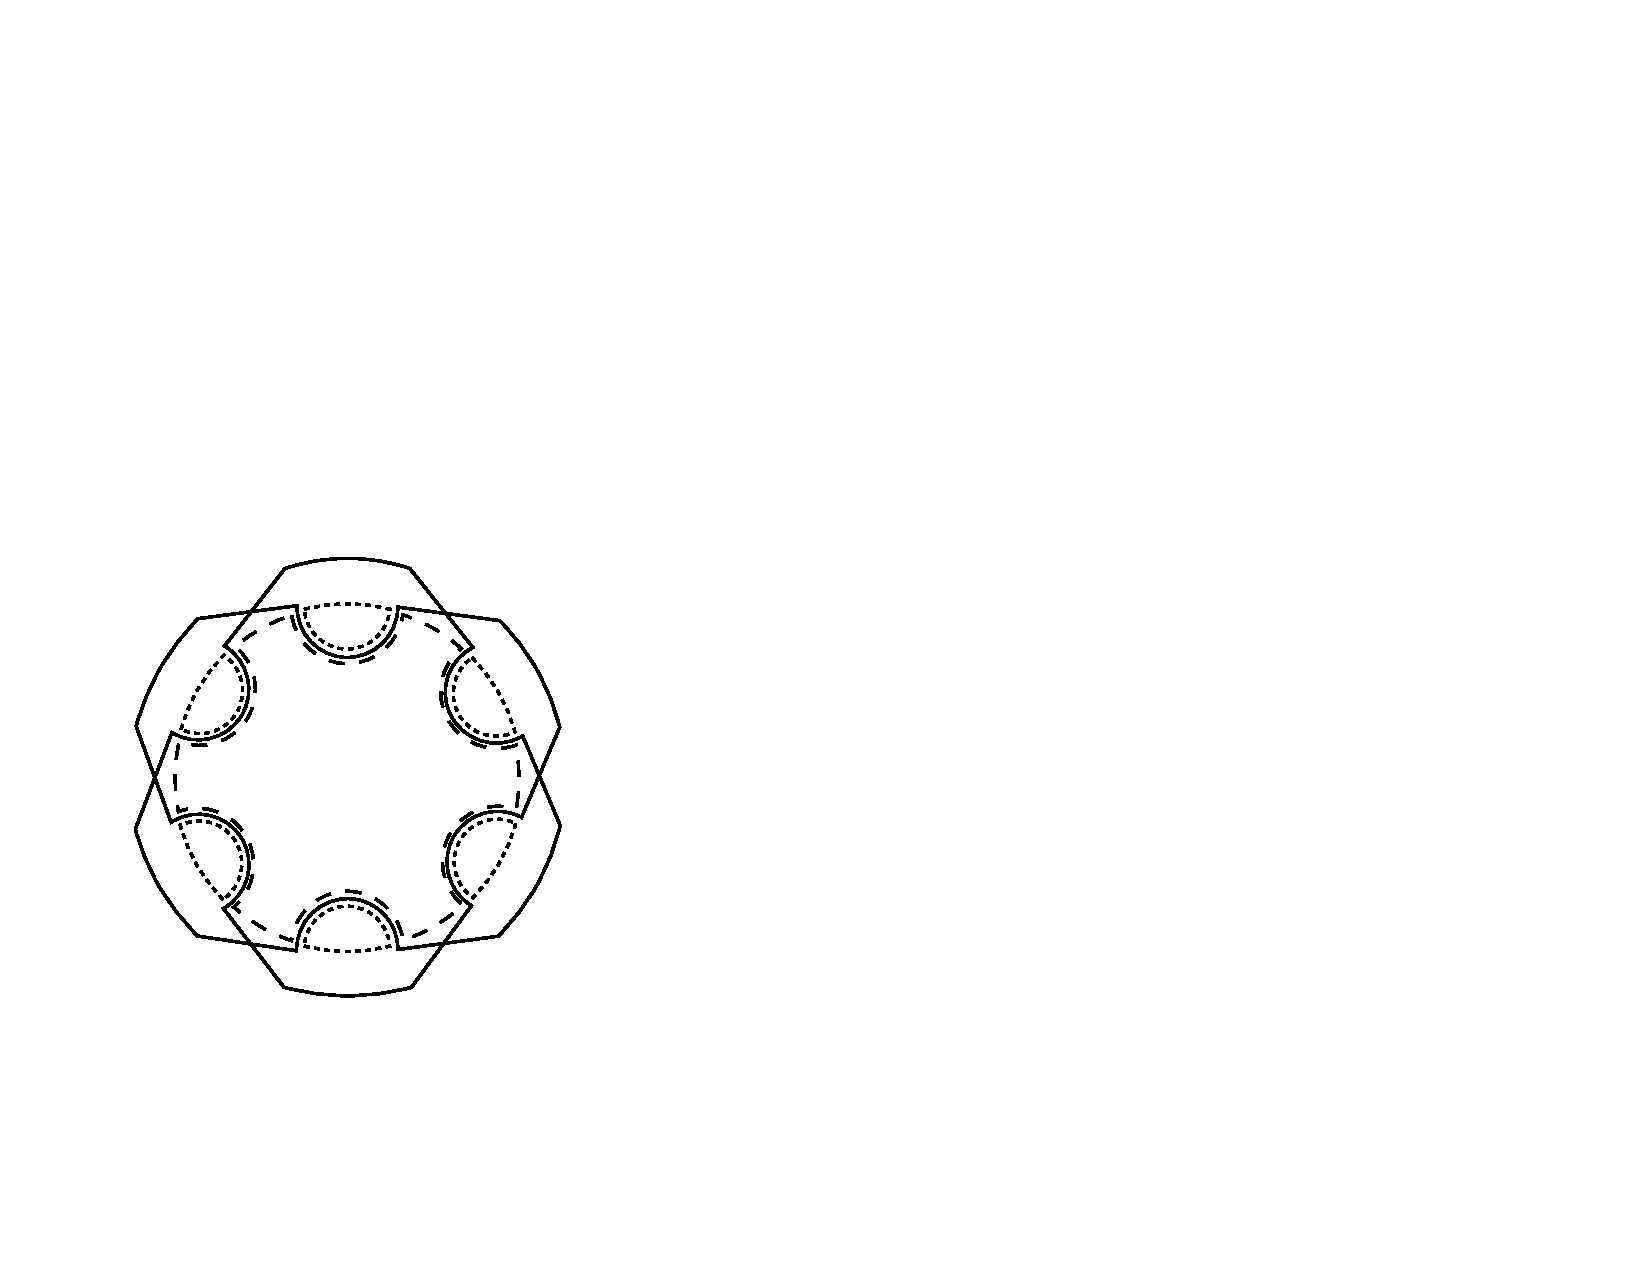
\includegraphics[scale=0.4]{images/RN6_A1large.pdf}}},
\end{align}
\begin{align}
    \vcenter{\hbox{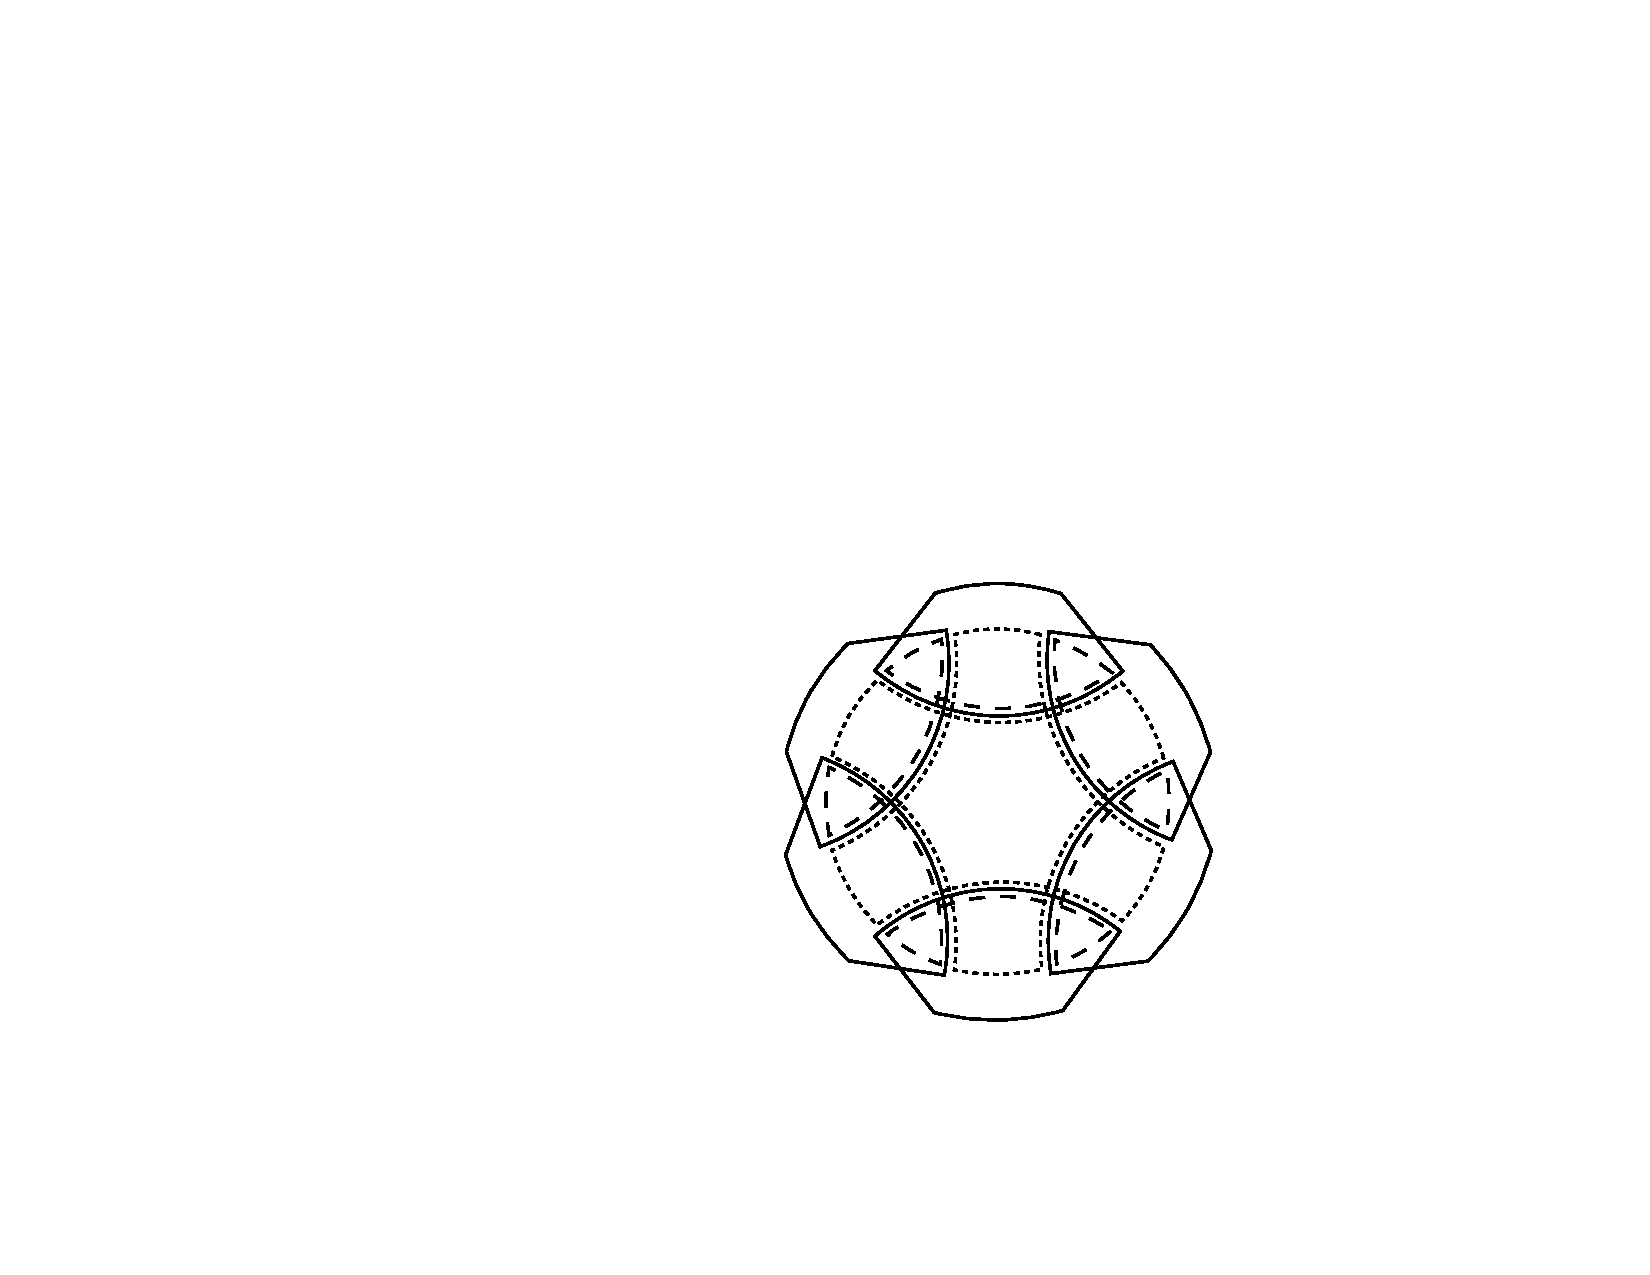
\includegraphics[scale=0.4]{images/RN6_A2large.pdf}}},
\end{align}

To sum up, This in turn implies that
\begin{align}
    \braket{\cal E} \approx \ 
    \left\{
    \begin{matrix}
    L_{B}^{1-n_e} L_{A_2}^{2-n_e} & \qquad  L_{A_1} \gg L_{A_2}
    \\
    \\
    L_{B}^{1-n_e} L_{A_1}^{2-n_e} & \qquad  L_{A_1} \ll L_{A_2}
    \end{matrix}
    \right.
\end{align}


\subsection{Resolvent function}

In this part, we derive Schwinger-Dyson equation for the negativity spectrum of a reduced density matrix of a random pure state.

We note that since there is an even/odd effect for the R\'enyi negativity, we need to consider two self-energy functions:
\begin{align}
G(z) = \frac{1}{z- \Sigma_1(z) - \Sigma_2(z)}
\end{align}
which satisfy
\begin{align}
\Sigma_1(z)  &= \alpha F_1(z), \\
\Sigma_2(z)  &= \beta F_2(z), 
\end{align}
where 
\begin{align}
\alpha = \frac{L_B}{L_{A_1}}, \qquad
\beta= \frac{L_B L_{A_2}}{L_{A_1}},
\end{align}
and
\begin{align}
F_2(z) = G(z)\cdot F_1(z) = \frac{G(z)}{1-G^2(z)}.
\end{align}
Solving for $G(z)$, we obtain the following cubic equation
\begin{align}
z G^3(z) + (\beta-1) G^2(z) + (\alpha -z ) G(z) +1 =0.
\end{align}
The proper solution to the above equation can be written as
\begin{align}
	a
\end{align}



\end{document}